% Source of QPool_report_zh_extended.pdf. Build in this folder with two runs of
%   xelatex -jobname=QPool_report_zh_extended main.tex
% (fonts: TeX Gyre Termes/Heros, STIX Two Math, Noto Serif CJK SC) and copy QPool_report_zh_extended.pdf to ../
\documentclass[a4paper,11pt]{article}
\usepackage{fontspec}
\setmainfont{TeX Gyre Termes}
\setsansfont{TeX Gyre Heros}
\newfontfamily\cjkfont{Noto Serif CJK SC}
\usepackage{amsmath}
\usepackage{unicode-math}
\setmathfont{STIXTwoMath-Regular.otf}
\usepackage[a4paper,top=2.5cm,bottom=2.4cm,left=2.6cm,right=2.6cm]{geometry}
\usepackage{graphicx,booktabs,array,threeparttable,pdfpages,fancyhdr,xurl}
\usepackage[font=small,labelsep=period,skip=4pt]{caption}
\usepackage[hidelinks,bookmarksnumbered=true,bookmarksopen=true]{hyperref}
\usepackage{titlesec}
\renewcommand{\floatpagefraction}{0.8}\renewcommand{\topfraction}{0.88}\renewcommand{\bottomfraction}{0.7}\renewcommand{\textfraction}{0.1}
\usepackage{etoolbox}\AtBeginEnvironment{thebibliography}{\small\linespread{1.05}\selectfont\setlength{\itemsep}{1pt}\setlength{\parskip}{0pt}}
\setlength{\emergencystretch}{3em}
\linespread{1.15}
\setlength{\parskip}{0.25em}
\titleformat{\section}{\large\bfseries}{E\arabic{section}}{0.8em}{}
\titleformat{\subsection}{\normalsize\bfseries}{E\arabic{section}.\arabic{subsection}}{0.6em}{}
\renewcommand{\thesection}{E\arabic{section}}
\renewcommand{\thefigure}{E\arabic{figure}}
\renewcommand{\thetable}{E\arabic{table}}
\renewcommand{\theequation}{E\arabic{equation}}
\setlength{\headheight}{15pt}\pagestyle{fancy}\fancyhf{}\renewcommand{\headrulewidth}{0.4pt}
\newcommand{\hd}[1]{\begin{tabular}[b]{@{}c@{}}#1\end{tabular}}
\newcommand{\exthead}[1]{\fancyhead[L]{\small #1}\fancyhead[R]{\small Part II\quad Post-competition extensions}\fancyfoot[C]{\small E-\thepage}}

\graphicspath{{../../figures/extension/}}
\hypersetup{pdftitle={QPool: quantum-classical dispatch for dynamic ride-pooling -- extended edition}}
\begin{document}
\thispagestyle{empty}
\begin{center}
{\Large\bfseries QPool: Quantum--Classical Co-Scheduling\\[0.2em] for Dynamic Ride-Pooling}\\[0.7em]
{\large Extended edition --- note}
\end{center}
\vspace{0.8em}

This file has two parts. Part I is the technical report submitted to the 1st Quantum Computing Application Scenario Challenge (university track), 2026 (12 pages, in Chinese), reproduced exactly as submitted. Part II, starting on page E-1, contains post-competition extensions written in November 2026.

The report validates the pipeline \emph{conflict-graph QUBO, exact reduction, 8-bit precision fitting, solution on the SPQC-550 device, equal-energy polish} on 6 frozen dispatch periods. Part II extends the test to every period recorded during the classical replays and answers two questions the report could not. E1 uses MILP to characterise exactly how 8-bit quantisation affects 435 periods: the hardware bottleneck is the int8 coefficient range rather than the number of spins, and the classical equal-energy polish cuts the worst-case quantisation loss from 1\,554 to 15 vehicle-minutes. E2 raises demand density to 1--12.5 times that of the public trace. From four times the density on, the reduced problems reach thousands of variables, far beyond the 549 usable spins of the device, while a classical exact solver proves the optimum of all 1\,331 periods within 1.8 s.

Every number in Part II can be reproduced with the scripts in the \texttt{extension/} folder of the code repository; result files are in \texttt{results/extension/}. The public Sioux Falls demand trace is subject to an upstream licence and must be downloaded as described in the repository.

\clearpage
\pdfbookmark[0]{Part I\quad Competition report (as submitted)}{part1}

\includepdf[pages=-]{../QPool_report_zh.pdf}
\pdfbookmark[0]{Part II\quad Post-competition extensions}{part2}
\setcounter{page}{1}
\exthead{QPool: quantum--classical co-scheduling for ride-pooling}
\begin{center}{\Large\bfseries Part II\quad Post-competition extensions}\end{center}

The report takes service-feasible vehicle trips as decision units and writes single-period dispatch as a weighted set-packing QUBO on a conflict graph. After exact reduction and 8-bit precision fitting the QUBO is solved on the SPQC-550 device, and the original business utility then selects among the solutions that tie after quantisation. The device experiments of the report cover 6 frozen periods. The two extensions below apply the same pipeline, without changing any model or parameter, to a large number of periods from real replays: E1 measures exactly the loss caused by quantisation itself, and E2 examines how problem size relates to device capacity as demand becomes denser.

\section{How much real dispatch can an 8-bit device carry? An exact quantisation audit}

\subsection{Method}
All 435 frozen periods recorded during the classical replays (8 combinations of fleet size and period length) pass through the same compilation as in the report: exact reduction, decomposition into connected components, choice of the scaling factor $\rho$ on a ladder of power-of-two resolutions, and a check of whether each component fits the SPQC-550 with signed 8-bit couplings. For every component that fits, MILP computes three quantities exactly: the optimum of the original problem, the optimum of the quantised problem, and the range of the original utility over all optima of the quantised problem. The last quantity gives the best and the worst result that an ideal Ising solver could legitimately return, which turns the quantisation error from an approximate estimate into an exactly computable interval.

\subsection{Results}
Exact reduction alone solves most periods: 295 of the 435 periods (68\,\%) have no free variable left after reduction, and the median number of free variables after reduction is 0. The combinatorial cores that reach the device are small, with a median of 5 variables per component and at most 138 at usable precision. The number of spins is not the bottleneck: all 178 non-trivial components have at most 257 variables, far below 549. What binds is the int8 coefficient range. Nine components, all from the replays with 32 and 48 vehicles, fit the device only with $\rho<1$, where most rounded weights become zero. Counted by whole periods, 100\,\% of the periods compile with $\rho\geq 1$ for 8 to 16 vehicles, 100\,\% (60-s periods) and 96\,\% (300-s periods) for 32 vehicles, and 98\,\% and 74\,\% for 48 vehicles; the remaining periods need the conditional-neighbourhood mode that the report uses for its snapshots A05 and A06.

Quantisation rarely loses the original optimum, but it often creates ties. In 40\,\% of the components that fit, the quantised problem has tied solutions with different original costs. The best solution in the quantised tie set equals the original optimum in 97.6\,\% of the components, whereas the worst admissible tied solutions together cost 1\,554 planned vehicle-minutes more. The report's classical equal-energy polish closes exactly this gap: starting from the worst tied solution, it reaches the best tied solution in 99.4\,\% of the components and reduces the total loss from 1\,554 to 15 vehicle-minutes (Figure~\ref{fig:qp-e1}). The a-priori bound $K/\rho$ given in the report is a median 7.8 times larger than the actual worst-case tie loss, and is therefore conservative.

\begin{figure}[htbp]\centering
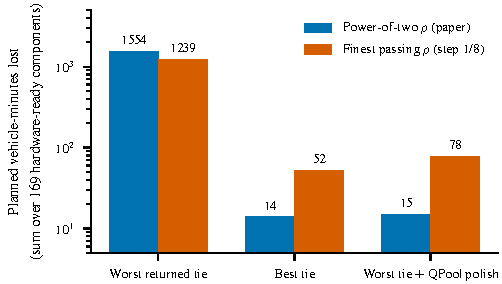
\includegraphics[width=0.52\textwidth]{figE1_quantization_loss.pdf}
\caption{Loss in planned vehicle-minutes caused by 8-bit quantisation (sum over the 169 deployable components of the 435 frozen periods, logarithmic scale). Blue: the report's power-of-two resolution; orange: the finest feasible resolution on a grid of step 1/8.}\label{fig:qp-e1}
\end{figure}

Finer resolution is not monotonically better. Searching for the finest feasible $\rho$ on a grid of step 1/8 lowers the worst-case tie loss from 1\,554 to 1\,239 but raises the loss after polish from 15 to 78. Paired by component, the finer resolution after polish is better in 4 components, worse in 7 and equal in 158. The reason is that re-rounding can push the original optimum out of the quantised tie set, and no post-processing can recover a solution that is not in the set. In a pipeline with a polish step, the property to protect is therefore that the original optimum stays inside the quantised tie set, not merely the size of the rounding error.

\section{Does the dispatch core outgrow the device as demand becomes denser?}

\subsection{Design}
The demand level of E1 is that of the report: 240 requests in about 1.9 hours of the public Sioux Falls trace. Real cities have denser demand. E2 replays the same classical dispatch at 1, 2, 4, 8 and 12.5 times the demand density: the first $240k$ requests of the trace are taken and their arrival times divided by $k$, so that the time span stays at about 1.9 hours; the fleet scales with demand to $16k$ or $32k$ vehicles, and the period length is 60 s or 300 s, which gives 20 replays with 1\,331 frozen periods. Each period is analysed as in E1: exact reduction, connected components, whether each component fits the SPQC-550 with $\rho\geq 1$, and the exact optimum and LP-relaxation bound computed with HiGHS\cite{huangfu2018}.

The report's reduction routine rescans the whole period after every deletion; a period with 972 candidates takes 34 s, and single periods of the densest replays exceed 20\,000 candidates. E2 therefore implements an event-driven version of the same reduction rule. For each pair of adjacent vertices it maintains the number of vertices in the closed neighbourhood of one that do not belong to that of the other, and dominance means that this count is zero. Deleting a vertex can only decrease the counts between its neighbours and their neighbours by one, so only vertices whose count drops to zero or that lose all their neighbours need to be re-examined. A work list dequeued by smallest index guarantees that every step deletes exactly the vertex the original routine would delete. On all 907 periods with at most 600 candidates and on 300 random instances, the new and the old routines return identical kept, fixed and deleted sets, and on the period with 972 candidates the new routine needs only 0.07 s.

\subsection{Results}
Table~\ref{tab:qp-e2} gives the range over the four fleet and period combinations at each density, and Figure~\ref{fig:qp-e2} the results of each replay.

\begin{table}[htbp]\centering\small\setlength{\tabcolsep}{5pt}
\caption{Results of the demand-density extension (ranges over the four fleet and period combinations at each density; ``deployable'' means that every component fits the SPQC-550 with $\rho\geq1$).}\label{tab:qp-e2}
\begin{tabular}{crrrrr}\toprule
\hd{Density\\$k$} & \hd{Requests /\\vehicles} & \hd{Solved by\\reduction} & \hd{Largest component\\(variables)} & \hd{Deployable\\periods} & \hd{Longest\\MILP (s)}\\\midrule
1 & 240 / 16--32 & 4--91\,\% & 25--167 & 96--100\,\% & 0.01\\
2 & 480 / 32--64 & 4--69\,\% & 109--984 & 13--98\,\% & 0.01--0.09\\
4 & 960 / 64--128 & 0--29\,\% & 412--2929 & 4--89\,\% & 0.02--0.13\\
8 & 1920 / 128--256 & 0--1\,\% & 1404--11126 & 0--62\,\% & 0.08--0.76\\
12.5 & 3000 / 200--400 & 0--4\,\% & 5317--24458 & 0--16\,\% & 0.50--1.79\\\bottomrule
\end{tabular}
\end{table}

\begin{figure}[htbp]\centering
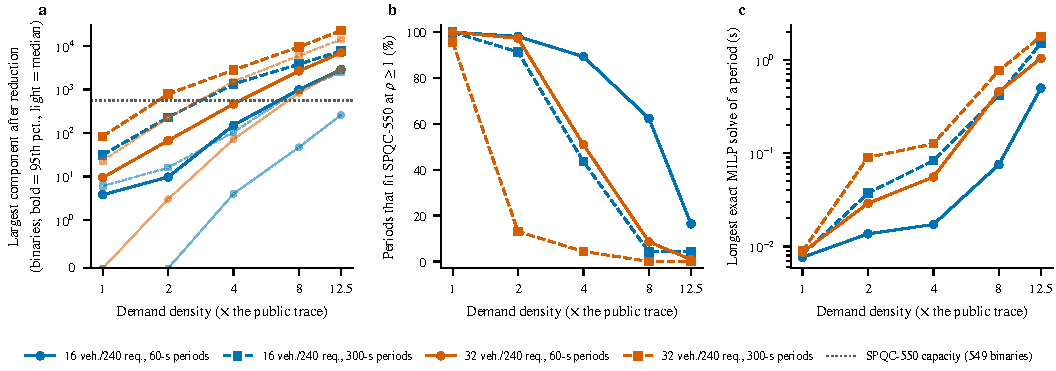
\includegraphics[width=0.9\textwidth]{figE2_density_scaling.pdf}
\caption{(a) Largest connected component after reduction per period as a function of demand density (thick lines: 95\,\% quantile; thin lines: median); the dashed line is the capacity of the SPQC-550. (b) Share of periods in which every component fits the device with $\rho\geq1$. (c) Longest exact MILP solution time of a single period.}\label{fig:qp-e2}
\end{figure}

The device carries the report's demand level, but not much more. At $k=1$ every component of almost every period fits the device; from $k=4$ on, the largest component after reduction reaches thousands of variables, whereas the device has 549 usable spins. For the larger fleets, the share of 60-s periods that still fit falls from 51\,\% at $k=4$ to 9\,\% at $k=8$, and the share of 300-s periods is at most 4\,\%. Exact reduction loses its power at the same time: at $k=1$ it solves 70\,\% to 91\,\% of the 60-s periods outright, at $k\geq 8$ at most 4\,\%; on average it deletes 83\,\% of a period's candidates at $k=1$ but only 35\,\% at $k=12.5$.

In contrast, the growth in problem size causes classical exact solution almost no difficulty. HiGHS proves the optimum of all 1\,331 periods, the slowest in 1.8 s; the LP relaxation is integral in 75\,\% of the periods, and its relative gap to the optimum never exceeds 7.5\,\%.

\subsection{Conclusions and limits}
At city-scale demand densities the quantum route is limited by spin capacity, and this limit appears long before the problem becomes hard for classical exact solution. The mode the report uses for its two largest snapshots, decomposition into device-sized conditional neighbourhoods, would have to carry almost the whole load at high density, and it should be the focus of further work in this direction. Each configuration was replayed with a single random seed, and denser demand was obtained by compressing the arrival times of the same public trace rather than by observing higher demand.

\begin{thebibliography}{9}
\bibitem{huangfu2018} Q. Huangfu, J. A. J. Hall. Parallelizing the dual revised simplex method. \emph{Mathematical Programming Computation}, 10(1): 119--142, 2018. doi:10.1007/s12532-017-0130-5.
\end{thebibliography}
\end{document}
